\documentclass{exam}

\usepackage{tikz}
\usetikzlibrary{decorations.pathmorphing}

\pagestyle{headandfoot}
\firstpageheader{Name:\underline{\hspace{100pt}}}{}{Date:\underline{\hspace{100pt}}}
\runningheader{}{\textbf{The Aetherius Olympiad in Mathematics}}{}
\firstpagefooter{}{\thepage}{}
\runningfooter{}{\thepage}{}

\begin{document}

\begin{center}
	\LARGE{\textbf{The Aetherius Olympiad in Mathematics}}

	\vspace{8pt}

	\large{2024-09}
\end{center}

\section*{Questions}

\begin{questions}
	\question[7]{
		There are two villages on one side of the river. One person from village A wants to go fishing at the river front, then go to village B to visit his friend. The direct distance from village A to the river is $250m$ and from village B to the river is $360m$. What is the minimum distance that person has to travel? Let the horizontal distance between A to B be $500m$.
		\begin{center}
			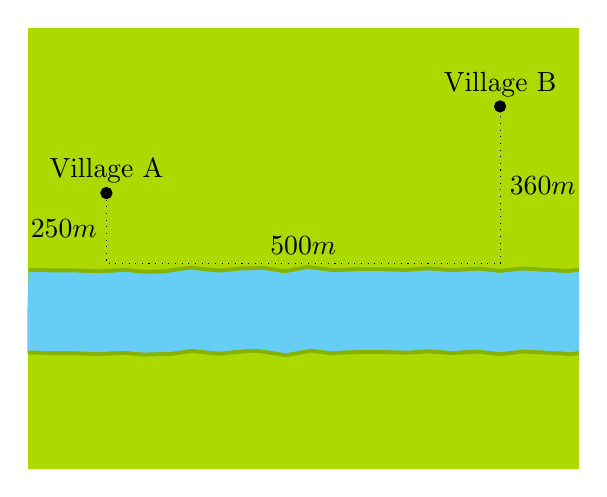
\begin{tikzpicture}
				\coordinate (LB) at (-1,-1);
				\coordinate (LT) at (-1,4.6);
				\coordinate (RB) at (6,-1);
				\coordinate (RT) at (6,4.6);
				\coordinate (Village A) at (0,2.5);
				\coordinate (Village B) at (5,3.6);

				\clip(LB)rectangle(RT);
				\fill[lime!70!olive] (LB)rectangle(RT); % background
				\pgfmathsetseed{14159}
				\draw[decorate, decoration={random steps, segment length=3mm, amplitude=1pt}, lime!70!black, line width=.5mm, double=cyan!60!white, double distance=1cm] (-1,1) -- (9,1); % river
				\draw[black, dotted] (Village A)--node[left]{$250m$}(0,1.6)--node[above]{$500m$}(5,1.6)--node[right]{$360m$}(Village B);
				\filldraw[black] (Village A) circle (2pt) node[anchor=south]{Village A};
				\filldraw[black] (Village B) circle (2pt) node[anchor=south]{Village B};
			\end{tikzpicture}
		\end{center}
	}
	\question[7]{$2024(2024^{2024})=?$

		Adapted from AMC 12 2000 Problem 2
	}
	\question[7]{
		How many positive integers $b$ have the property that $\log_{b} 729$ is a positive integer?

		From AMC 12 2000 Problem 7
	}
	\question[7]{
	Given a group of numbers (called an arithmetic series) $S_n=a_1+a_2+\dots+a_n$, show that $S_n=\frac{n}{2}(2a_1+(n-1)d)$ where $d=a_i-a_{i-1}$ for all $2 \leq i \leq n$.
	}
	\question[7]{
		In triangle $\triangle ABC$, points E, F, and G are on the line $\overline{AB}$, $\overline{BC}$, and $\overline{AC}$, respectively. If $\frac{AE}{BE} \cdot \frac{BF}{CF} \cdot \frac{CG}{AG} = 1$, prove that $\overline{CE}$, $\overline{AF}$, and $\overline{BG}$ intersect at a distinct point.
	}
	\question[7]{
	Given a triangle $\triangle KAI$, let $\overline{HK_1}=a$ and $\overline{H_1I}=b$, find $\sum_{n=1}^{\infty} H_nH_{n-1}$.
	}
\end{questions}

\end{document}
